\documentclass[11pt, oneside]{article}   	% use "amsart" instead of "article" for AMSLaTeX format
\usepackage{geometry}              		% See geometry.pdf to learn the layout options. There are lots.
\usepackage{amsmath}
\geometry{letterpaper}                   		% ... or a4paper or a5paper or ... 
%\geometry{landscape}                		% Activate for rotated page geometry
%\usepackage[parfill]{parskip}    		% Activate to begin paragraphs with an empty line rather than an indent
\usepackage{graphicx}				% Use pdf, png, jpg, or eps§ with pdflatex; use eps in DVI mode
								% TeX will automatically convert eps --> pdf in pdflatex		
\usepackage{amssymb}

%SetFonts

%SetFonts


\title{Homework 1}
\author{Weiyu Yan}
\date{}							% Activate to display a given date or no date

\begin{document}
\maketitle
\section{Perceptron Algorithm and Convergence Analysis}

\begin{enumerate}
\item	%1
  \begin{enumerate}
  \item	%a
    weight vector is $w=(-1,0)$ \\
    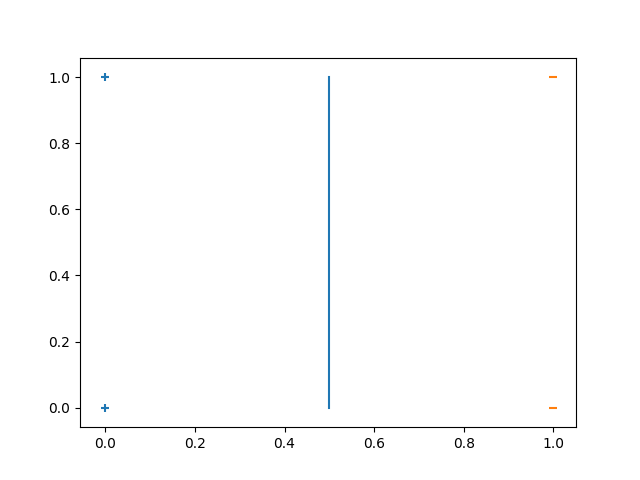
\includegraphics[width=15cm]{1_1a.png}\\
  \item	%b
    A truth table for this function could be:\\
    \begin{tabular}{|c|c|c|}
      \hline
      $x_1$ & $x_2$ & $y$ \\ \hline
      0     & 0     & 1   \\ \hline
      0     & 1     & 0   \\ \hline
      1     & 0     & 0   \\ \hline
      1     & 1     & 1   \\ \hline
    \end{tabular}\\
    We can plot those points in a figure.\\
    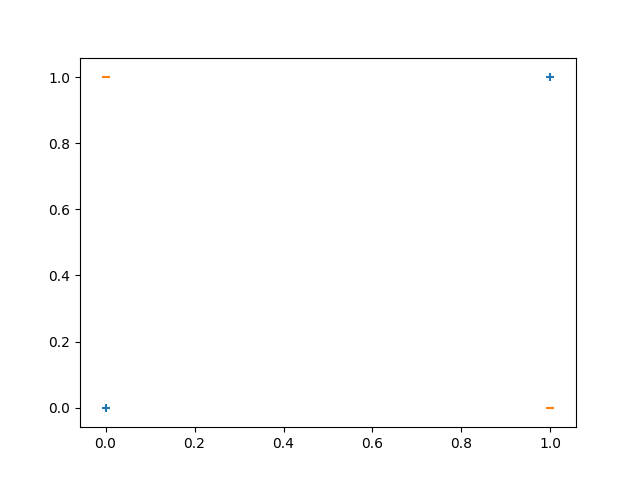
\includegraphics[width=15cm]{1_1b.png}
    The perceptron algorithm gives us a weight vector which corresponds to its orthogonal hyperplane to divide points into 2 parts. In this figure since we can't find a hyperplane to divide the 2 kinds, this function can't be represented by a single perceptron.
  \item	%c
    weight vector is $w=(0,0,-1)$\\
    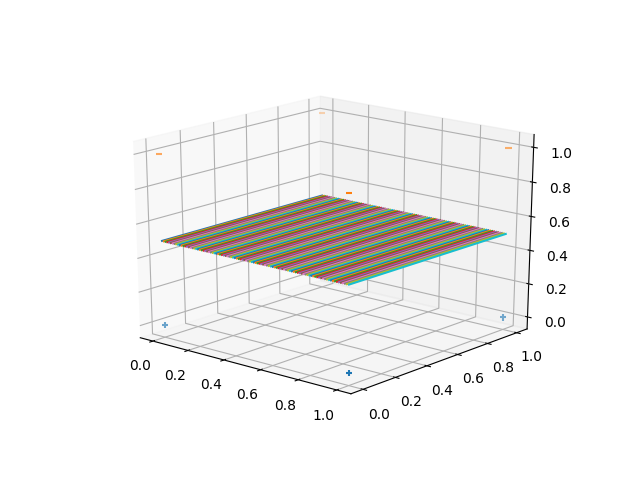
\includegraphics[width=15cm]{1_1c.png}\\
  \end{enumerate}

\item %2
  $\beta$ is a weight vector perpendicular to the hyperplane
  the signed Euclidean Distance of the point $x$ to the hyperplane is given by:
  \[
  d=\frac{(x-x_0) \cdot \beta y} {\left \| \beta \right \|_2}\\
  \]
  where
  \[
  x_0 \in \{x|f(x)=0\}
  \]
  \[
  \because f(x_0)=\beta_0 + \beta^Tx_0
  \]
  \[
  \therefore \beta^T x_0 = -\beta_0
  \]
  Therefore
  \begin{equation}
    \begin{split}
      d&=\frac{y(x \cdot \beta - x_0 \cdot \beta)} {\left \| \beta \right \|_2}\\
      &=\frac{y(\beta^T x - \beta^T x_0)} {\left \| \beta \right \|_2}\\
      &=\frac{y(\beta^T x + \beta_0)} {\left \| \beta \right \|_2}\\
      &=\frac{yf(x)} {\left \| \beta \right \|_2}
    \end{split}
  \end{equation}

\item %3
  \begin{equation}
    \begin{split}
        & \| w^T - w^{sep} \|^2 \\
      = & \| (w^{T-1} + x_i y_i) - w^{sep} \|^2 \\
      = & \| w^{T-1} + x_i y_i \|^2  + \| w^{sep} \|^2 - 2 (w^{T-1} + x_i y_i) w^{sep} \\
      = & \|w^{T-1}\|^2 + \|x_i y_i\|^2 + 2 w^{T-1} x_i y_i + \| w^{sep} \|^2 - 2 w^{T-1} w^{sep} - 2 x_i y_i w^{sep}   \\
    \end{split}
  \end{equation}
  
  \[
  \because
  \| w^{T-1} - w^{sep} \|^2 = \|w^{T-1}\|^2 +  \| w^{sep} \|_2^2 - 2 w^{T-1} w^{sep}
  \]
  \[
  \therefore
  \| w^T - w^{sep} \|^2 - \| w^{T-1} - w^{sep} \|^2 = \|x_i y_i\|^2 + 2 w^{T-1} x_i y_i - 2 x_i y_i w^{sep}
  \]

since the weight vector only updates when making a mistake, we have:
\[
w^{T-1} x_i y_i \leq 0 \\
\]
Also for the algorithm we persume:
$ \|x_i y_i\|^2 \leq 1 $ and $ x_i y_i w^{sep} \geq 1 $\\
We can derive:
\begin{equation}
  \begin{split}
   & (\| w^T - w^{sep} \|^2 - \| w^{T-1} - w^{sep} \|^2) \\
    &+ (\| w^{T-1} - w^{sep} \|^2 - \| w^{T-2} - w^{sep} \|^2) + \cdots \\
    &+  (\| w^1 - w^{sep} \|^2 - \| w^0 - w^{sep} \|^2) \\
    &= \| w^T - w^{sep} \|^2 - \| w^0 - w^{sep} \|^2
    \leq \sum_{t=1}^{T}-1 = -T
  \end{split}
\end{equation}
Therefore,
\[
0 \leq \| w^T - w^{sep} \|^2 \leq \| w^0 - w^{sep} \|^2 - T 
\]
\[
\therefore T \leq \| w^0 - w^{sep} \|^2 
\]

\end{enumerate}


\section{Programming Assignment}
Please refer code in 'hw1.py'
\begin{enumerate}
\item	%1
  \begin{enumerate}
  \item	%a
    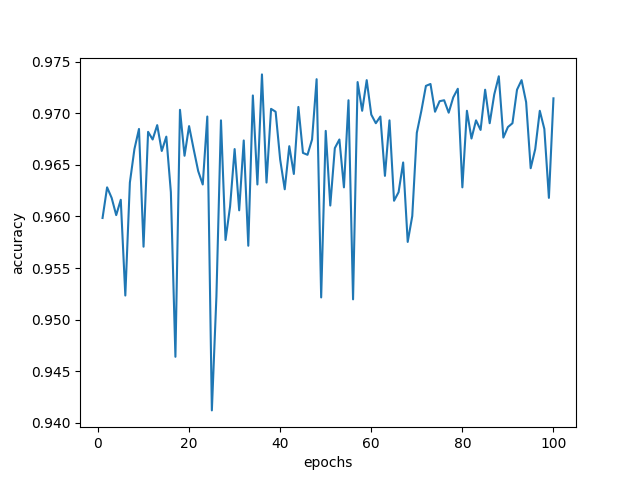
\includegraphics[width=15cm]{2_1a.png}\\
    Since first epoch the accuracy is already pretty good.\\
    Then it shakes drastically at first(within a small bound, in general the accuracy is always above 0.94), then becomes more steady, with the moving average increasing slowly.\\
    By increasing/decreasing number of epochs, the curve becomes denser/sparser -- just revealing more/less information in the figure, the points' location won't change.
  \item	%b
    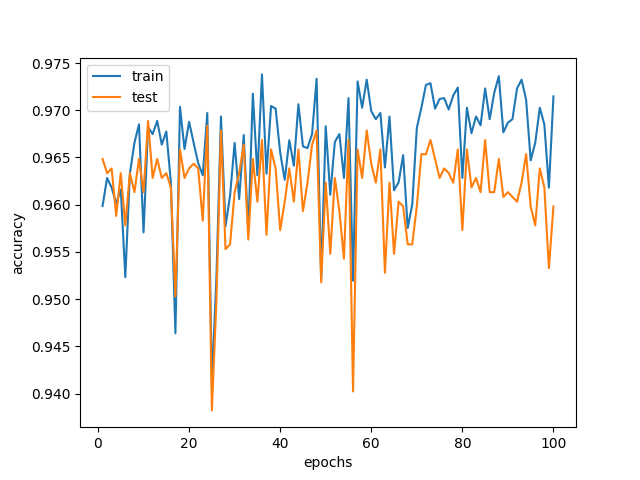
\includegraphics[width=15cm]{2_1b.png}\\
    The curve for test set roughly follows the same pattern of traning set. With the epoch number going up,  it becomes lower than the training set.
  \item	%c
    accuracy: 0.9598191863385234\\
    confusion matrix:
    \[
    \left[
      \begin{array}{cc}
	965	&	38\\
	44	&	944
      \end{array}
      \right]
    \]
  \item %d
    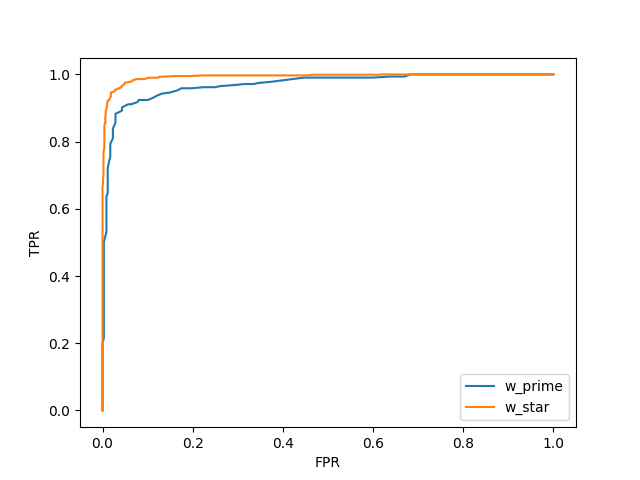
\includegraphics[width=15cm]{2_1d.png}
  \item %e
    AUC($ w^\prime) = 0.9698776549779418$\\
    AUC($ w^*) = 0.9937542766829695$\\
    The greater the AUC value, the bigger area that is under the ROC curve, the 'upper' that the ROC curve goes.
  \end{enumerate}

\item %2
  \begin{enumerate}
  \item
    Accuracy evolution for training set with $eta=0.05$ after 30 epochs:\\
    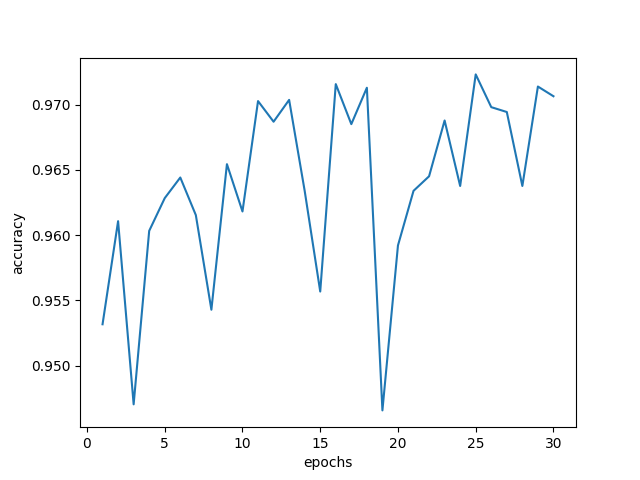
\includegraphics[width=15cm]{2_2a.png}
    For test set:\\
    accuracy: 0.9658463083877449\\
    confusion matrix:
    \[
    \left[
      \begin{array}{cc}
	982	&	41\\
	27	&	941
      \end{array}
      \right]
    \]

  \item
    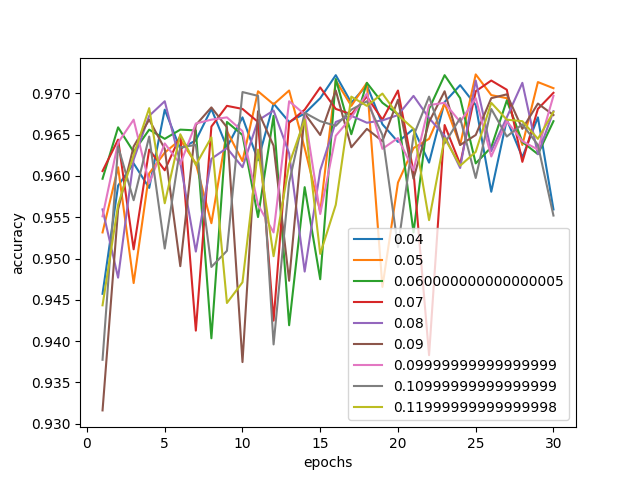
\includegraphics[width=15cm]{005wins.png}
    The technique I use is to first plot accuracy curves using small epoch numbers and look for a smaller range of this best $\eta$, I presume $argmax(f(\eta))$ is a convex function with local min being its global min. Then I wrote a loop to plot curves with better precision in this small range. Observe from the figure that $\eta \approx 0.05$ is the best value in my experiment.


    
  \end{enumerate}
\end{enumerate}






\end{document}  
